\documentclass{article}
\usepackage{leonine,amsmath,amssymb,amsthm,graphicx,setspace}%%xy, setspace, amscd (commutative diagram)
\title{Notes}
\author{Eric Purdy \footnote{Department of Computer Science, University of Chicago. Email: epurdy@uchicago.edu}}

%%\doublespace

\begin{document}
\maketitle

\setcounter{section}{0}

\section{Assembling Datasets} 

\section{Grammatical Shape Models}
% hand_built.tex

\marginnote{beginning of models/hand\_built.tex}

\subsection{Build an interesting grammar by hand}
\marginnote{Should probably do hand here?}

\marginnote{Move this experiment to the section on building a grammar
  from a single curve.}

Here we are drawing a grammar. We have built this grammar by hand, by
taking the following curve, and specifying a decomposition of it:

\begin{figure}
\includegraphics[width=\linewidth]{experiments/1.grammars/hand_built/output.d/hand_built_curve.png}
\caption{The initial curve}
\end{figure}

Here is the decomposition:
\begin{figure}
\includegraphics[width=\linewidth]{experiments/1.grammars/hand_built/output.d/hand_built_sdf.png}
\end{figure}

Here is the grammar:

\begin{figure}
Here are some samples from the grammar:


\includegraphics[width=6in]{output/3.learning/incremental/gram.30.d/samples.png}


\end{figure}

\marginnote{end of models/hand\_built.tex}


\section{Parsing}

\FloatBarrier

\section{Recovering a One-to-one Correspondence}

Here we have two curves given by hand-annotation of the Romer
dataset. We build a grammar from the curve on the left, using a
hand-built set of constituents. We then parse the curve on the right,
and show the Viterbi parse by showing the correspondences between the
two curves.

Because there are no missing or extra points, this is straightforward.

\begin{figure}
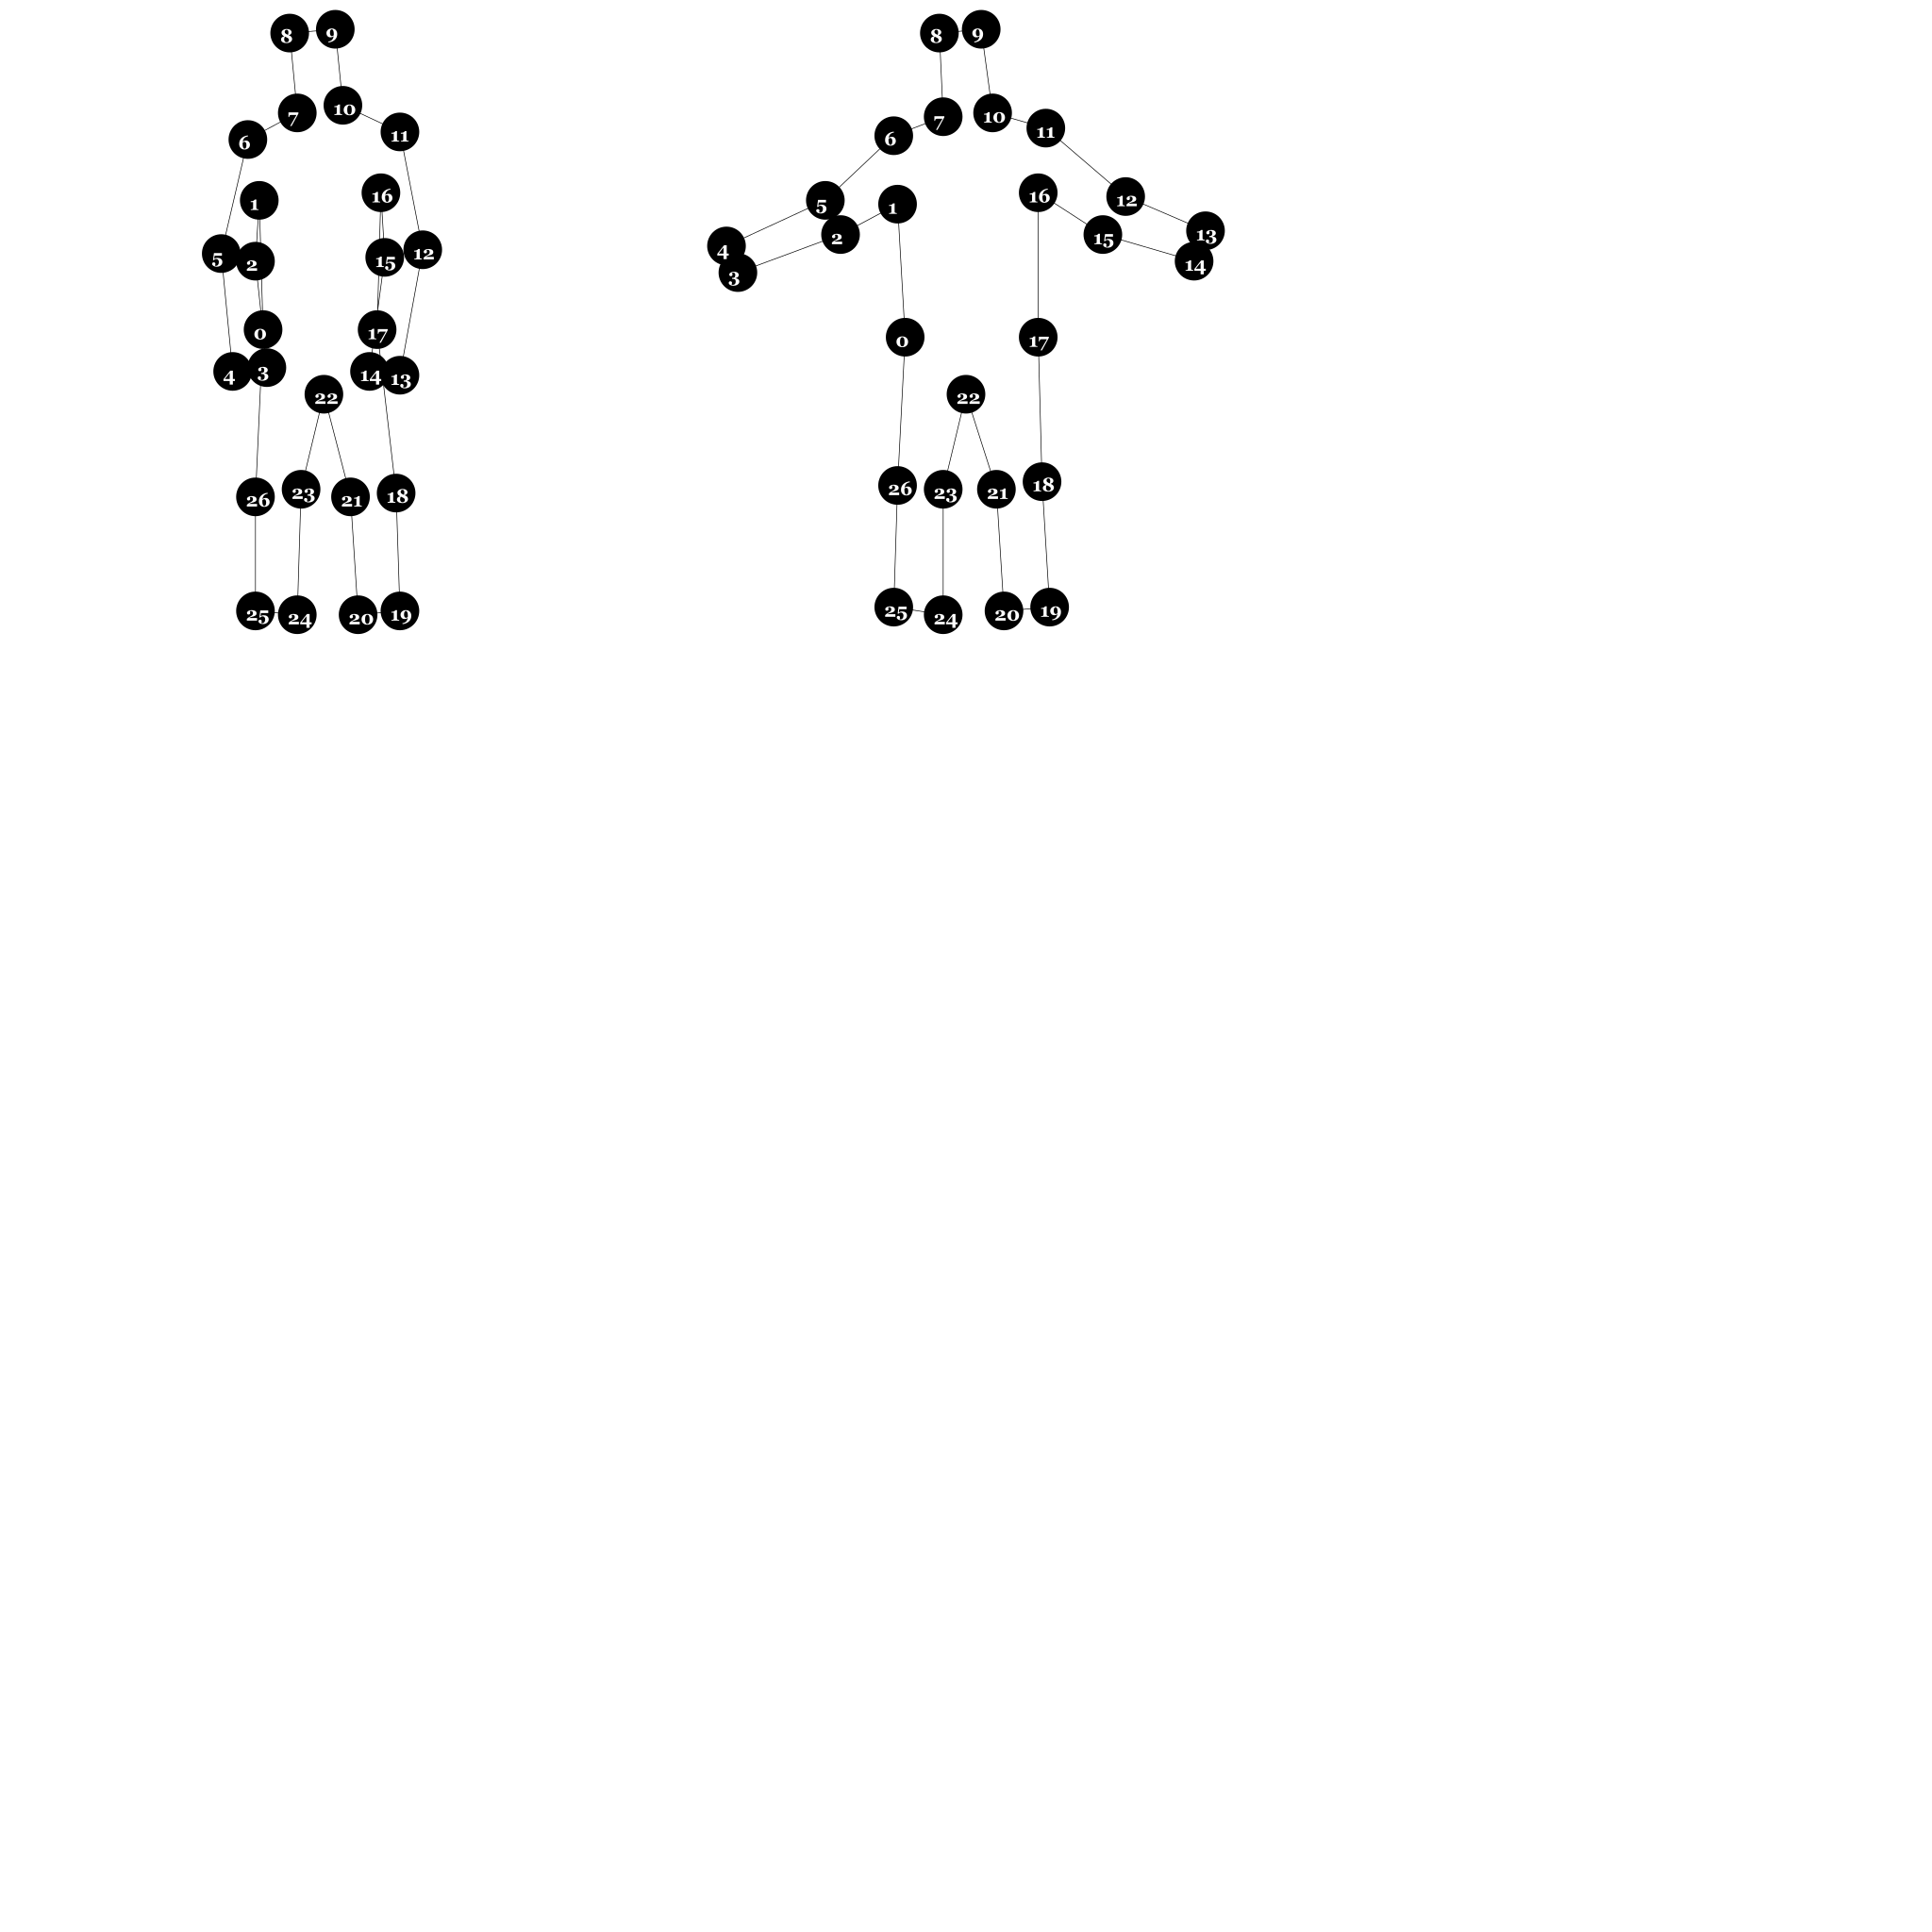
\includegraphics[width=\linewidth]{experiments/2.parsing/one_to_one/output.d/parse.png}
\caption[Recovering a One-to-one Correspondence]{On the left, the model curve. On the right, the parsed curve}
\end{figure}


\section{EM}

\subsection{Simple tuning}

Here is our example curve, from which we build a grammar with hand-chosen rules.

\includegraphics[width=2in]{./3.em/simple_tuning/examples.eps}

Here are our training curves:

\includegraphics[width=2in]{./3.em/simple_tuning/training.eps}

Here is the grammar:

\subsubsection{Initial}
Here are some samples from the grammar:


\includegraphics[width=6in]{output/3.learning/incremental/gram.30.d/samples.png}



\subsubsection{Round 1}
Here are some samples from the grammar:


\includegraphics[width=6in]{output/3.learning/incremental/gram.30.d/samples.png}


\subsubsection{Round 2}
Here are some samples from the grammar:


\includegraphics[width=6in]{output/3.learning/incremental/gram.30.d/samples.png}


\subsubsection{Round 3}
Here are some samples from the grammar:


\includegraphics[width=6in]{output/3.learning/incremental/gram.30.d/samples.png}


\subsubsection{Round 4}
Here are some samples from the grammar:


\includegraphics[width=6in]{output/3.learning/incremental/gram.30.d/samples.png}


\subsubsection{Round 5}
Here are some samples from the grammar:


\includegraphics[width=6in]{output/3.learning/incremental/gram.30.d/samples.png}




\section{Parsing in Cluttered Images}

\section{Using SDF's in Other Domains}

\section{Learning Structure}


\subsection{Learning Good Constituents}

We use explicit correspondences to learn the statistically best set of
constituents when building a grammar from a single example.

Note that the arms are found as constituents!

%% we can use \input{} here to incorporate dynamically generated text

\includegraphics[width=5in]{./6.structure/constituents/constituents.eps}



\section{Learning Texture}

\begin{figure}
\includegraphics[width=0.45\linewidth]{experiments/7.texture/scaled_nts/output.d/scaled_nts_training_1.png}
\hfill
\includegraphics[width=0.45\linewidth]{experiments/7.texture/scaled_nts/output.d/scaled_nts_1.png}
\\\vspace{3\baselineskip}
\includegraphics[width=0.45\linewidth]{experiments/7.texture/scaled_nts/output.d/scaled_nts_training_2.png}
\hfill
\includegraphics[width=0.45\linewidth]{experiments/7.texture/scaled_nts/output.d/scaled_nts_2.png}
\\\vspace{3\baselineskip}
\includegraphics[width=0.45\linewidth]{experiments/7.texture/scaled_nts/output.d/scaled_nts_training_3.png}
\hfill
\includegraphics[width=0.45\linewidth]{experiments/7.texture/scaled_nts/output.d/scaled_nts_3.png}
\\\vspace{3\baselineskip}
\includegraphics[width=0.45\linewidth]{experiments/7.texture/scaled_nts/output.d/scaled_nts_training_4.png}
\hfill
\includegraphics[width=0.45\linewidth]{experiments/7.texture/scaled_nts/output.d/scaled_nts_4.png}
\\\vspace{3\baselineskip}
\includegraphics[width=0.45\linewidth]{experiments/7.texture/scaled_nts/output.d/scaled_nts_training_5.png}
\hfill
\includegraphics[width=0.45\linewidth]{experiments/7.texture/scaled_nts/output.d/scaled_nts_5.png}
\caption{Training on left, samples on right.}
\end{figure}

\begin{figure}
\includegraphics[width=0.45\linewidth]{experiments/7.texture/scaled_nts/output.d/scaled_nts_training_6.png}
\hfill
\includegraphics[width=0.45\linewidth]{experiments/7.texture/scaled_nts/output.d/scaled_nts_6.png}
\\\vspace{3\baselineskip}
\includegraphics[width=0.45\linewidth]{experiments/7.texture/scaled_nts/output.d/scaled_nts_training_7.png}
\hfill
\includegraphics[width=0.45\linewidth]{experiments/7.texture/scaled_nts/output.d/scaled_nts_7.png}
\\\vspace{3\baselineskip}
\includegraphics[width=0.45\linewidth]{experiments/7.texture/scaled_nts/output.d/scaled_nts_training_8.png}
\hfill
\includegraphics[width=0.45\linewidth]{experiments/7.texture/scaled_nts/output.d/scaled_nts_8.png}
\\\vspace{3\baselineskip}
\includegraphics[width=0.45\linewidth]{experiments/7.texture/scaled_nts/output.d/scaled_nts_training_9.png}
\hfill
\includegraphics[width=0.45\linewidth]{experiments/7.texture/scaled_nts/output.d/scaled_nts_9.png}
\\\vspace{3\baselineskip}
\includegraphics[width=0.45\linewidth]{experiments/7.texture/scaled_nts/output.d/scaled_nts_training_10.png}
\hfill
\includegraphics[width=0.45\linewidth]{experiments/7.texture/scaled_nts/output.d/scaled_nts_10.png}
\caption{Training on left, samples on right.}
\end{figure}

\begin{figure}
\includegraphics[width=0.45\linewidth]{experiments/7.texture/scaled_nts/output.d/scaled_nts_training_11.png}
\hfill
\includegraphics[width=0.45\linewidth]{experiments/7.texture/scaled_nts/output.d/scaled_nts_11.png}
\\\vspace{3\baselineskip}
\includegraphics[width=0.45\linewidth]{experiments/7.texture/scaled_nts/output.d/scaled_nts_training_12.png}
\hfill
\includegraphics[width=0.45\linewidth]{experiments/7.texture/scaled_nts/output.d/scaled_nts_12.png}
\\\vspace{3\baselineskip}
\includegraphics[width=0.45\linewidth]{experiments/7.texture/scaled_nts/output.d/scaled_nts_training_13.png}
\hfill
\includegraphics[width=0.45\linewidth]{experiments/7.texture/scaled_nts/output.d/scaled_nts_13.png}
\\\vspace{3\baselineskip}
\includegraphics[width=0.45\linewidth]{experiments/7.texture/scaled_nts/output.d/scaled_nts_training_14.png}
\hfill
\includegraphics[width=0.45\linewidth]{experiments/7.texture/scaled_nts/output.d/scaled_nts_14.png}
\\\vspace{3\baselineskip}
\includegraphics[width=0.45\linewidth]{experiments/7.texture/scaled_nts/output.d/scaled_nts_training_15.png}
\hfill
\includegraphics[width=0.45\linewidth]{experiments/7.texture/scaled_nts/output.d/scaled_nts_15.png}
\caption{Training on left, samples on right.}
\end{figure}


\end{document}